\documentclass{article}
\usepackage{tikz}
\usetikzlibrary{arrows.meta,positioning,calc,shapes.geometric}
\pagestyle{empty}
\begin{document}
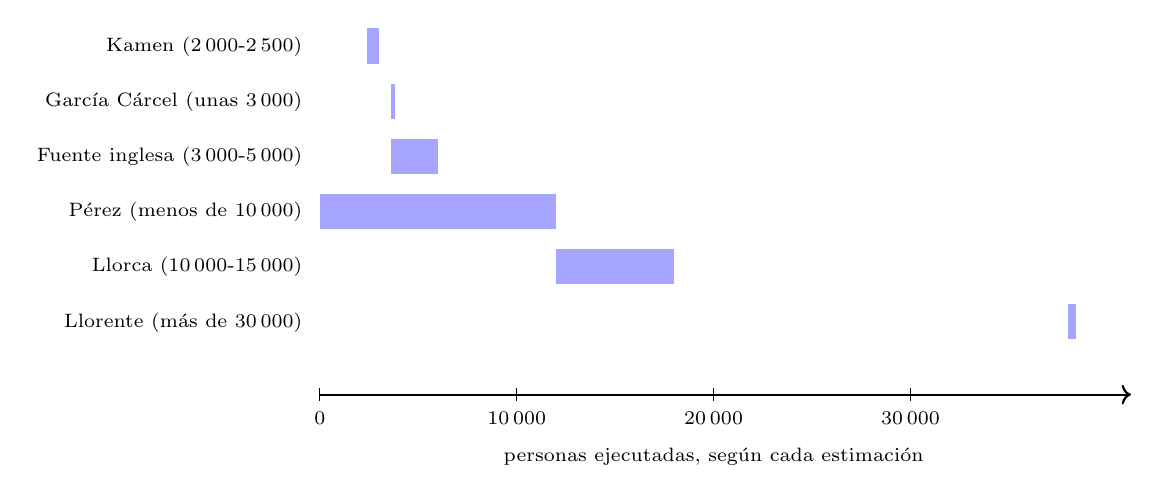
\begin{tikzpicture}

\draw[->, thick] (0,0) -- (10.3,0);
\foreach \x/\l in {0/0,2.5/10\,000,5/20\,000,7.5/30\,000} { \draw (\x,-0.08) -- (\x,0.08); \node[font=\scriptsize, anchor=north] at (\x,-0.1) {\l}; }
\node[font=\scriptsize, anchor=north] at (5,-0.55) {personas ejecutadas, según cada estimación};
\def\row#1#2#3#4{ \fill[blue!35] (#2,#1) rectangle (#3,#1+0.45); \node[font=\scriptsize, anchor=east] at (-0.1,#1+0.22) {#4}; }
\row{4.2}{0.6}{0.75}{Kamen (2\,000-2\,500)}
\row{3.5}{0.9}{0.95}{García Cárcel (unas 3\,000)}
\row{2.8}{0.9}{1.5}{Fuente inglesa (3\,000-5\,000)}
\row{2.1}{0}{3.0}{Pérez (menos de 10\,000)}
\row{1.4}{3.0}{4.5}{Llorca (10\,000-15\,000)}
\row{0.7}{9.5}{9.6}{Llorente (más de 30\,000)}

\end{tikzpicture}
\end{document}
